\chapter{Requirement Analysis}
\label{chap:requirement-analysis}

\section{Stakeholder Analysis}
\label{section:stakeholder-analysis}

% \section*{Key Stakeholders and Their Roles}

\subsection{Primary Target Users (Direct Beneficiaries)}
These stakeholders directly interact with TaskAlign and gain the most benefits from its scheduling optimization features.

\textbf{Factory Managers} – Oversee production operations and seek efficient scheduling methods to reduce downtime and optimize machine utilization.

\textbf{Production Planners} – Responsible for task scheduling and workforce allocation, ensuring production efficiency and minimizing bottlenecks.

\textbf{Machine Operators \& Technicians} – Directly interact with machinery and rely on TaskAlign for clear, optimized schedules to streamline manual operations.

\subsection{Secondary Target Users (Indirect Beneficiaries)}
These stakeholders benefit from TaskAlign’s impact but do not use the system as actively as the primary users.

\textbf{Factory Owners} – Interested in cost-effective solutions that improve productivity without requiring expensive equipment upgrades.

\textbf{IT \& System Administrators} – Manage the implementation and integration of TaskAlign with existing factory systems, including ERP solutions.

\textbf{Supply Chain \& Logistics Teams} – Depend on optimized production schedules for better coordination of raw material procurement and order fulfillment.

\textbf{Customers \& Clients} – Indirect stakeholders who benefit from reduced lead times, improved production efficiency, and consistent product availability.

TaskAlign addresses the needs of these stakeholders by providing an optimized, data-driven scheduling system tailored to solve small to medium electronic factories that are still reliant on manual scheduling in manufacturing environments.


\section{User Stories}
\label{section:user-stories}

% //#TODO: place table here
% \begin{figure}[h]
%     \centering
%     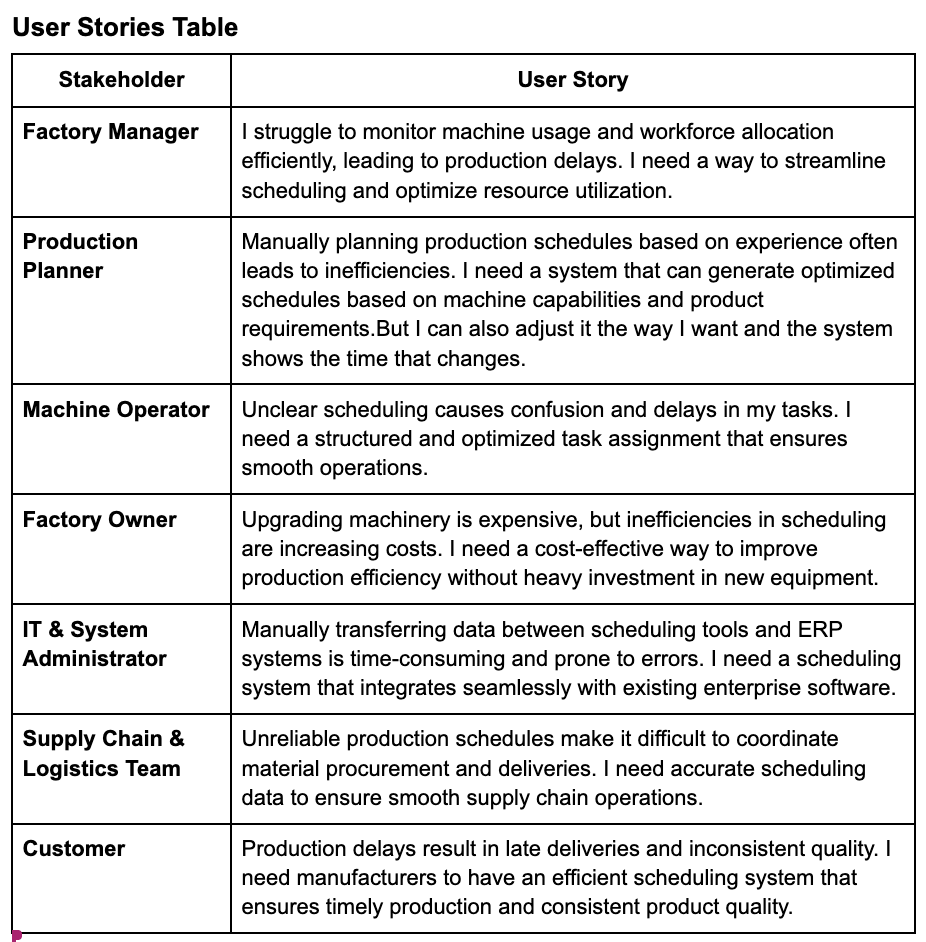
\includegraphics[width=0.5\textwidth]{examples/user_story.png}
%     \caption{User Story Table} 
% \end{figure}
\begin{table}[!h]
    \begin{adjustwidth}{-.85in}{-.85in}
        \noindent
        \centering
        \small\begin{tabularx}{1.3\textwidth}{|>{\columncolor{yellow!20}\raggedright\arraybackslash}p{2.5cm}|X|}
            \hline
            \textbf{Stakeholder} & \textbf{User Story} \\\hline
            Factory Manager & I struggle to monitor machine usage and workforce allocation efficiently, leading to production delays. I need a way to streamline scheduling and optimize resource utilization. \\\hline
            Production Planner & Manually planning production schedules based on experience often leads to inefficiencies. I need a system that can generate optimized schedules based on machine capabilities and product requirements. But I can also adjust it the way I want and the system shows the time that changes. \\\hline
            Machine Operator & Unclear scheduling causes confusion and delays in my tasks. I need a structured and optimized task assignment that ensures smooth operations. \\\hline
            Factory Owner & Upgrading machinery is expensive, but inefficiencies in scheduling are increasing costs. I need a cost-effective way to improve production efficiency without heavy investment in new equipment. \\\hline
            IT \& System Administrator & Manually transferring data between scheduling tools and ERP systems is time-consuming and prone to errors. I need a scheduling system that integrates seamlessly with existing enterprise software. \\\hline
            Supply Chain \& Logistics Team & Unreliable production schedules make it difficult to coordinate material procurement and deliveries. I need accurate scheduling data to ensure smooth supply chain operations. \\\hline
            Customer & Production delays result in late deliveries and inconsistent quality. I need manufacturers to have an efficient scheduling system that ensures timely production and consistent product quality. \\\hline
        \end{tabularx}
    \end{adjustwidth}
    \caption{User Stories by Stakeholder}
\end{table}



\section{Use Case Diagram}
\label{section:use-case-diagram}
<TIP: Write a use case diagram for your project here. Refer to an
article “What is a use case diagram?” by Lucidchart for help./>

\section{Use Case Model}
\label{section:use-case-model}
A use case is a detailed description of how a system
interacts with an external entity (such as a user or another system) to
accomplish a specific goal. Use cases provide a high-level view of the
functionality of a system and help in capturing and documenting its
requirements from the perspective of end users.

<TIP: Write use cases for your project here. Make sure to use the
appropriate type of use case for each scenario (brief, casual, and fully-dressed
use case)./>

\section{User Interface Design}
\label{section:user-interface-design}
<TIP: Put the initial design of your application here. You can
showcase a detailed design of a specific page or a sitemap of your application.
See an example below./>

\begin{figure}[h]
    \centering
    \includegraphics[width=0.8\textwidth]{examples/user-interface-design.png}
    \caption{User Interface Design}
\end{figure}